\documentclass[a4paper, 12pt]{article}
\usepackage[left=1.8cm,right=1.8cm,top=2cm,bottom=2cm]{geometry}

\usepackage[T1]{fontenc}
\usepackage[utf8]{inputenc}
\usepackage{etex,amsfonts,amssymb,amsmath,mathrsfs}
\usepackage{dsfont}
\usepackage{pifont}
\usepackage[tikz]{bclogo}
\usepackage{tikz,tkz-tab}
\usetikzlibrary{arrows,shadows,shapes,backgrounds,positioning,lindenmayersystems}
\usepackage{fancyhdr}
\usepackage{fancybox}
\setlength{\headheight}{12.81pt}
\usepackage[french]{babel}
\DecimalMathComma
\frenchbsetup{StandardLists=true}
\usepackage{lmodern}
\usepackage{xspace}
\usepackage[francais]{layout}
\usepackage{textcomp} %Pour simple quote droit \textquotesingle
\usepackage{fourier-orns}
\usepackage{colortbl}
\usepackage{multicol}
\usepackage{multirow}
\usepackage{numprint}
\usepackage{multido}
\usepackage{ifthen}
%%%%%%%%%%%%%%%%%%%%%%%%%%%%%%%%%%%%%%%%%%%%%%%%%%%%%%%%%%%%%%
\usepackage[french,lined,vlined,linesnumbered]{algorithm2e}
% \usepackage[french,lined,vlined,linesnumbered,boxed]{algorithm2e}
\setlength{\algomargin}{1em}
%%%%%%%%%%%%%%%%%%%%%%%%%%%%%%%%%%%%%%%%%%%%%%%%%%%%%%%%%%%%%%
\usepackage{stmaryrd}
\SetSymbolFont{stmry}{bold}{U}{stmry}{m}{n}
\usepackage{alltt}
\usepackage{moreverb}
\usepackage{appendix}

%%%%%%%%%%%%%%%%%%%%%%%%%%%%%%%%%%%%%%%%%%%%%%%%%%%%%%%%%%%%%%
%%%%%%%%%%%%%%%%%%%%%%%%%%%%%%%%%%%%%%%%%%%%%%%%%%%%%%%%%%%%%%

\usepackage{cellspace}
% Pour régler l'espacement vertical des filets et du texte dans un tableau
% \cellspacetoplimit=3pt
% \cellspacebottomlimit=3pt
% écrire Sc pour une colonne centrée

%%%%%%%%%%%%%%%%%%%%%%%%%%%%%%%%%%%%%%%%%%%%%%%%%%%%%%%%%%%%%%
%%%%%%%%%%%%%%%%%%%%%%%%%%%%%%%%%%%%%%%%%%%%%%%%%%%%%%%%%%%%%%

\graphicspath{{images/}}

%%%%%%%%%%%%%%%%%%%%%%%%%%%%%%%%%%%%%%%%%%%%%%%%%%%%%%%%%%%%%%
%%%%%%%%%%%%%%%%%%%%%%%%%%%%%%%%%%%%%%%%%%%%%%%%%%%%%%%%%%%%%%

% \renewcommand{\textbf}[1]{\begingroup\bfseries{\mathversion{bold}#1}\endgroup}
\usepackage{varwidth} 
\usepackage{setspace}
\usepackage{amsmath}
\usepackage{fancybox, graphicx}
\usepackage{color}
\usepackage{hyperref}
\pagestyle{fancy}
\renewcommand{\footrulewidth}{1pt}
\fancyfoot[L]{La Pr\'epa des INP - Bordeaux}
\fancyfoot[C]{\thepage}
\fancyfoot[R]{Ann\'ee universitaire 2019-2020}
\fancyhead[L]{\leftmark}
\fancyhead[C]{}
\fancyhead[R]{Ondes acoustiques dans les fluides}

\begin{document}

\begin{titlepage}
{
\includegraphics[height=1.5cm]{bx-inp.eps}}
{
\includegraphics[height=1.5cm]{cpp-inp.eps}}
\vspace*{\stretch{1}}
\begin{center}
 \Huge{\textbf{Cours d'ondes acoustiques dans les fluides}}
\end{center}
\vspace*{\stretch{0.25}}
\begin{center}
 \normalsize{Axel MATAVAR - Alexandre CHOURA - Etienne LEMESLE}
\end{center}
\vspace*{\stretch{0.25}}
\begin{center}
 {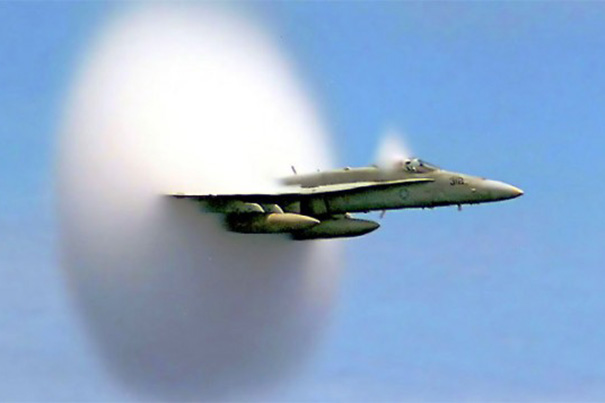
\includegraphics[scale=0.65]{frst-pg.eps}}
\end{center}
\vspace*{\stretch{1}}
\begin{center}
 \Large{\textit{Ann\'ee universitaire 2019-2020}}
\end{center}
\vspace*{\stretch{1}}
\end{titlepage}

\tableofcontents
\newpage

\section{Mise en équation des ondes sonores}

\subsection{Introduction}

L'objectif de ce projet est, dans un premier temps, de montrer que la propagation du son est un phénomène ondulatoire, puis d'essayer de décrire cette propagation dans les fluides qualitativement et quantitativement.\newline \newline
Par exemple, un haut parleur émet du son dans l'air. L'air étant un fluide déformable, il se déforme lors du passage du son, entraînant une modification de volume (et donc de masse volumique et de pression) pour les particules de fluide voisines. Cette déformation se propage ensuite jusqu'à atteindre notre oreille par exemple, créant ainsi une onde \underline{acoustique}.
\begin{flushright}
{\textcolor{blue}{\href{https://youtu.be/px3oVGXr4mo?t=09}{Observation d'un "clap" par strioscopie}}}
\end{flushright}
Pour l'étude on retiendra ceci:
\begin{itemize}
\item Les ondes sonores sont des ondes mécaniques: elles nécessitent un milieu matériel pour se propager (on peut d'ailleurs montrer par l'expérience que le son est inaudible dans le vide).

\item Étudier les ondes acoustiques traversant le fluide revient donc à étudier les perturbations qu'elles causent dans le fluide. C'est-à-dire que l'on tentera de mettre en équation les variations de pression et le déplacement des particules de fluides.
\end{itemize}

\subsection{Position des hypothèses}
\subsubsection{Approximation acoustique}
Le fluide étudié est considéré parfait et on néglige l'influence de la pesanteur.\newline
Nous caractérisons le fluide au repos par:
\begin{itemize}
\item une pression uniforme $P_0$,
\item une masse volumique uniforme $\mu_0$,
\item une vitesse particulaire nulle (à différencier de la vitesse de l'onde!).
\end{itemize}
L'onde sonore constitue \textbf{une perturbation par rapport à cet état d'équilibre}. On décrit alors l'état du fluide dans l'espace et dans le temps par:
\begin{itemize}
\item la pression $P(M,t)=P_0+p(M,t)$, où $p(M,t)$ est la surpression due au passage de l'onde (\underline{pression acoustique}),
\item la masse volumique $\rho_{tot}(M,t)=\rho_0+\rho(M,t)$, avec $\rho(M,t)$ la variation de masse volumique,
\item $\vec{v}(M,t)$ la vitesse des particules de fluide induite par la propagation des ondes acoustiques. \newline
\end{itemize}
Pour notre étude, nous aurons besoin des approximations suivantes dans le cadre des petites déformations:$\begin{cases}
|p(M,t)|\ll P_0 &\text{(1)}\\
|\rho(M,t)|\ll \rho_0 \text{, le fluide reste relativement incompressible} \\
||\vec{v}(M,t)||\ll c \text{, où c est la vitesse de l'onde} &\text{(2)}
\end{cases}$\newline \newline \newline
L'hypothèse (1) se vérifie par l'expérience. Effectivement, pour les ondes acoustiques on peut mesurer la pression acoustique créée. Prenons un cas extrême : le décollage d'une fusée engendre {\textcolor{blue}{\href{https://fr.wikipedia.org/wiki/Comparaison_du_volume_de_sources_courantes_de_bruit}{une pression acoustique de $2.10^4$ Pa}}}(l'équivalent de 180 dB); ce qui reste négligeable devant la pression atmosphérique de $10^5$ Pa. Si on considère maintenant un son banal : une personne qui parle, l'ordre de grandeur est de $0,01$ Pa. Nous restons donc largement sous cette hypothèse. \newline
\begin{center}
{\includegraphics[height=4cm]{fusee.eps}}
\end{center}
L'hypothèse (3) se vérifiera plus tard (cf 4.3)\newline
\underline{Conclusion}: Par la suite, les petites grandeurs de variation que nous avons définies serons des termes d'ordre 1 par rapport auxquels on négligera \textbf{tous les termes d'ordre supérieur}.

\subsubsection{Approximation isentropique}
D'autres grandeurs comme la température entrent en jeu. Nous sommes donc amenés à faire des \textbf{hypothèses thermodynamiques} dans notre étude. En effet, l'onde acoustique peut se modéliser comme une succession de compressions du fluide qui se propagent. Dans un premier temps, nous négligerons les phénomènes irréversibles (viscosité du fluide, diffusion de particules notamment). En particulier, l'hypothèse (1) est cohérente car elle impose un faible gradient de pression au cours des transformations.\newline
On ajoute à cela l'hypothèse de transformations \textbf{adiabatiques} (cf 4.3), nous étudions alors des transformations \underline{isentropiques} ($\Delta S=0$). \newline \newline
On choisit alors de décrire le fluide par son \textbf{coefficient de compressibilité isentropique}:
\begin{center}
$\chi_S=-\frac{1}{V}{(\frac{\partial V}{\partial P})}_S$
\end{center}

\subsection{Équation de propagation}
On applique l'équation d'Euler au fluide supposé parfait:
\begin{center}
$\rho_{tot}(\frac{\partial \vec{v}(M,t)}{\partial t}+\underbrace{(\vec{v}.\overrightarrow{\textrm{grad}})\vec{v}(M,t)}_{\text{négligé car d'ordre 2 (cf 4.3)}})=-\overrightarrow{\textrm{grad}}P(M,t)$    : équation \textcircled{a}
\end{center}
Or, $P(M,t)=P_0+p(M,t)$\newline
\begin{center}
Donc, $\overrightarrow{\textrm{grad}}P(M,t)=\overrightarrow{\textrm{grad}}(\underbrace{P_0}_{cte}+p(M,t))$ \newline
	  $\overrightarrow{\textrm{grad}}P(M,t)=\overrightarrow{\textrm{grad}}\:p(M,t)$	
\end{center}
On a aussi
\begin{center}
$\rho_{tot}(M,t)\frac{\partial \vec{v}(M,t)}{\partial t}=\rho_0\frac{\partial \vec{v}(M,t)}{\partial t}+\underbrace{\rho(M,t)\frac{\partial \vec{v}(M,t)}{\partial t}}_{ordre 2}$\newline \newline
$\rho_{tot}(M,t)\frac{\partial \vec{v}(M,t)}{\partial t}\approx\rho_0\frac{\partial \vec{v}(M,t)}{\partial t}$
\end{center}
\textcircled{a} devient donc:
\begin{center}
\fbox{$\rho_0\frac{\partial \vec{v}(M,t)}{\partial t}=-\overrightarrow{\textrm{grad}}p(M,t)$    : \textcircled{a}}
\end{center}
L'équation de conservation de la masse en 3D nous donne:
\begin{center}
$\rho_{tot}(M,t)div\:\vec{v}(M,t)+\frac{\partial \rho_tot(M,t)}{\partial t}=0$    : équation \textcircled{b}
\end{center}
Simplifions de la même manière que précédemment:
\begin{center}
$\rho_{tot}(M,t)div\:\vec{v}(M,t)=\rho_0div\:\vec{v}(M,t)+\underbrace{\rho(M,t)div\:\vec{v}(M,t)}_{ordre 2}$\newline
$\rho_{tot}(M,t)div\:\vec{v}(M,t)\approx\rho_0div\:\vec{v}(M,t)$\newline \newline
Et $\frac{\partial \rho_{tot}(M,t)}{\partial t}=\frac{\partial (\overbrace{\rho_0}^{cte}+\rho(M,t))}{\partial t}=\frac{\partial \rho(M,t)}{\partial t}$
\end{center}
\textcircled{b} devient alors:
\begin{center}
\fbox{$\rho_0div\:\vec{v}(M,t)+\frac{\partial \rho(M,t)}{\partial t}=0$    : \textcircled{b}}
\end{center}
Introduisons maintenant $\chi_s$ dans les équations.\newline \newline
Par définition, $\chi_S=-\frac{1}{V}{(\frac{\partial V}{\partial P})}_S$
\begin{center}\begin{tabular}{ccl}
\vspace{2mm}
$\chi_S$	    &=& $-\frac{\rho_{tot}}{m}{(\frac{\partial (\frac{m}{\rho_{tot}})}{\partial P})}_S$\quad : on peut sortir la masse du fluide car celle-ci est constante\\
\vspace{2mm}
	            &=&	$\frac{\rho_{tot}}{\rho_{tot}^2}{(\frac{\partial \rho_{tot}}{\partial P})}_S$\quad car $\frac{\partial {(\frac{1}{x}})}{\partial P}=-\frac{1}{x^2}\frac{\partial x}{\partial P}$ \\
\vspace{2mm}
	            &=&	$\frac{1}{\rho_{tot}}{(\frac{\partial \rho_{tot}}{\partial P})}_S$\\
\vspace{2mm}
$\chi_S$	    &$\approx$&	$\frac{1}{\rho_0}{(\frac{\partial \rho_{tot}}{\partial P})}_S$\quad car$\rho_{tot}\approx\rho_0$    : \textcircled{c}
\end{tabular}\end{center}
Tentons d'exprimer ${(\frac{\partial \rho_{tot}}{\partial P})}_S$ en fonction des autres grandeurs.\newline
On peut choisir d'écrire toute grandeur thermodynamique en fonction d'un couple d'autres grandeurs. On choisit ici logiquement d'écrire $\rho_{tot}(P,S)$. En particulier, $\rho_0=\rho_{tot}(P_0,S)$.\newline
En appliquant la formule de Taylor à l'ordre 1, on obtient
\begin{center}
$\rho_{tot}(P,S)=\rho_{tot}(P_0+p,S)$\newline
$\rho_{tot}(P,S)\approx\underbrace{\rho_{tot}(P_0,S)}_{=\rho_0}+p{(\frac{\partial \rho_{tot}}{\partial P})}_S$\newline
Donc, $\rho_0+\rho=\rho_0+p{(\frac{\partial \rho_{tot}}{\partial P})}_S$\newline \newline
D'où $\rho=p{(\frac{\partial \rho_{tot}}{\partial P})}_S$ ou encore ${(\frac{\partial \rho_{tot}}{\partial P})}_S=\frac{\rho}{p}$\newline \newline
En reprenant \textcircled{c}, on arrive à\newline \newline
\fbox{$\rho=\chi_S\rho_0p$    : \textcircled{c}}
\end{center}
On peut maintenant appliquer \textcircled{a}, \textcircled{b}, \textcircled{c} afin d'obtenir une équation de propagation:\newline
On applique l'opérateur $div$ à l'équation \textcircled{a}
\begin{flushright}
Rappel : $div(\overrightarrow{\textrm{grad}})=\Delta$ et $div(\frac{\partial .}{\partial t})=\frac{\partial}{\partial t}(div\:.)$
\end{flushright}
\begin{center}
$\frac{\partial}{\partial t}(\rho_0div\:\vec{v}(M,t))=-\Delta p(M,t)$
\end{center}
Or, $\rho_0div\:\vec{v}(M,t)$ nous est donné par \textcircled{b}. On obtient donc
\begin{center}
$\frac{\partial}{\partial t}(-\frac{\partial \rho(M,t)}{\partial t})=-\Delta p(M,t)$\newline \newline
Donc, $\Delta p(M,t)-\frac{\partial^2 \rho(M,t)}{\partial t^2}=0$
\end{center}
Finalement, en appliquant \textcircled{c}

\noindent\shadowbox{\begin{minipage}[t]{1\linewidth}%
\begin{center}
$\Delta p(M,t)-\chi_S\rho_0\frac{\partial^2 p(M,t)}{\partial t^2}=0$\newline
$\Delta p(M,t)-\frac{1}{c^2}\frac{\partial^2 p(M,t)}{\partial t^2}=0$, où $c=\frac{1}{\sqrt{\rho_0\chi_S}}$
\end{center}
\underline{Remarque}: On retrouve une équation de d'Alembert similaire à celle établie en propagation des ondes mécaniques où $c$ est la célérité de l'onde dans le fluide.

\end{minipage}}

\section{Ondes sonores planes progressives}
\subsection{Ondes planes porgressives}
\begin{text}[]
Les équations précédentes ont toutes la même forme: elles sont linéaires à coefficients constants. Il est ainsi possible , grâce à l'analyse de Fourier, de décomposer la solution générale de ces équations en combinaisons linéaires d'ondes planes progressives.\newline
\left \{
\begin{array}{r c l}
p(x,y,z,t)=$f_{p}(t-\frac{\vec u\cdot\vec r}{c})+g_{p}(t+\frac{\vec u\cdot\vec r}{c})$\\
\rho(x,y,z,t)=$f_{\rho}(t-\frac{\vec u\cdot\vec r}{c})+g_{\rho}(t+\frac{\vec u\cdot\vec r}{c})$\\
\vec v(x,y,z,t)=$\vec f_{v}(t-\frac{\vec u\cdot\vec r}{c})+\vec g_{v})(t+\frac{\vec u\cdot\vec r}{c})$\\
 \end{array}
   \right .\newline
   \end{text}[]
   
   
\begin{text}
Le vecteur unitaire $\vect u$ précise la direction de propagation. En se limitant à une onde plane progressive harmonique (OPPH) de pulsation $\omega$, grandeur s précédantes s'écrivent:
\newline
   \left \{
   \begin{array}{r c l}
      p(x,y,z,t) = $p_{m}cos[\omega(t-\frac{\vec u\cdot\vec r}{c})]$\\
      \rho(x,y,z,t) = $\rho_{m}cos[\omega(t-\frac{\vec u\cdot\vec r}{c})]$\\
      vec v(x,y,z,t) = $vec v_{m}cos[\omega(t-\frac{\vec u\cdot\vec r}{c})]$\\
   \end{array}
   \right .
   \newline
\end{text}
\begin{text}

On pose alors le vecteur d'onde $\vec k$ = $\frac{\omega}{c}\vec u$. La linéarité des équations permet également d'adopter la réprésentation complexe: \newline
   \left \{
   \begin{array}{r c l}
      \underline{p}(x,y,z,t) = $p_{m}e^{j(\omega t - \vec k \cdot\vec r)}$\\
      \underline{\rho}(x,y,z,t) = $\rho_{m}e^{j(\omega t - \vec k \cdot\vec r)}$\\
      \vec \underline{v}(x,y,z,t) = $\vec v_{m}e^{j(\omega t - \vec k \cdot\vec r)}$\\
   \end{array}
   \right .
\end{text}
\subsection{Structure des ondes planes progressives}
\begin{text}
En écrivant la relation $\vec rot(\vec v)$ en représentation complexe , on obtient:\newline $-j\vec k \land \underline{\vec v}$ = $\vec O$.\newline
Le vecteur vitesse $\underline{\vec v}$ est donc colinéaire au vecteur d'onde $\vec k$, c'est à dire à la direction de propagation de l'onde. L'onde sonore est donc une onde longitudinale.\newline 
De manière générale, ce résultat reste vrai pour les ondes planes progressives en raison du caractère linéaire de la décomposition de Fourier. On peut donc retenir que les ondes sonores planes progressives sont longititudinales. 
\end{text}
\subsection{Impédance acoustique}

\begin{text}
Par analogie à l'impédance électrique, on définit l'impédance acoustique pour relier linéairement la différence entre deux états du fluide parcouru par l'onde sonore(surpression p) et le mouvement de matière qui en résulte (vitesse $\vec v$).
\end{text}
\begin{defn}[]
En représentation complexe, on définit l'impédance acoustique $\underline{Z}$ par:\newline 
$\underline{Z}$ = $\frac{\underline{P}}{\underline{v}}$\newline
avec $\underline{Z}$ l'impédance acoustique($kg\cdot m^{-2}\cdot s^{-1}$)\newline
$\underline{P}$ la surpression en pascal (Pa)\newline
$\underline{v}$ la vitesse ($m \cdot s^{-1}$)\newline
\end{defn}[]
\begin{text}
Pour une OPPH, l'équation d'Euler linéarisée en représentation complexe donne: \newline 
$j\omega \rho_{0}\vec \underline{v}$ = $j\vec k\underline{\rho}$.\newline

En projetant cette relation sur la direction de propagation $\vec u$, on obtient l'impédence:\newline 
$\underline{Z}$ = $-\rho{0}c$,\newline

les champs de supression et de vitesse vibrant alors en opposition de phase.\newline 
Pour une OPPH,l'impédance acoustique est réelle, indépendante de la pulsation $\omega$ et vaut:\newline
$|\underline{Z}|$ = $\rho_{0}c$ = $\sqrt{\frac{\rho_{0}}{\chi_{0}}}$\newline 

L'impédanceacoustique est donc d'autant plus élevée que le milieu est dense($\rho_{0}$ élevé) et peu compressible($\chi_{0}$ faible). De manière générale, ce résultat reste vrai pour les ondes planes progressives.
\end{text}
\subsection{ordres de grandeur et vitesse du son}
\begin{text}
La vitesse des ondes sonores s'écrit:\newline 
c=$\frac{1}{\sqrt{\rho_{0}\chi_{0}}}$, avec $\chi_{0}$=$\frac{1}{\rho_{0}}(\frac{\partial \rho}{\partial p})$.\newline 
Dans le cas d'un gaz parfait, on peut préciser l'expression du coefficient de compressibilité isentropique$\chi{0}$. L'équation d'une isentropique est en effet donnée par la loi de Laplace:\newline
p=$C\rho^{\gamma}$, où $\gamma$ désigne le coefficient isentropique.\newline 
En utilisant l'équation d'état des gaz parfait:\newline 
p=$\frac{\rho RT}{M}$, en utilisant la dérivé de la loi de Laplace et en injectant la loi des gaz parfaits on obtient:\newline 
$\chi_{0}$=$\frac{M}{\gamma \rho_{0}RT_{0}}$.\newline 
Dans le cas des gaz parfaits, la vitesse c des ondes sonores a pour expression:\newline 
c=$\sqrt{\frac{\gamma R T_{0}}{M}}$\newline 
avec: c la vitesse ($m\cdot s^{-1}$)\newline
$\gamma$ coefficient isentropique\newline 
R=8,31 ($Jmol^{-1}K^{-1}$) la constante des gaz parfaits.\newline $T_{0}$ température en kelvin (K)\newline 
M masse molaire ($kg\cdot mol^{-1})$\newline 

A temperature ambiante:\newline 
$T_{0}$ = 298 K\newline 
c= 345 $m\cdot s^{-1}$
Z = 403 $kg.m^{-2}s^{-1}$

\end{text}
\section{Aspect énergétiques}
\subsection{Densité de courant d'énergie}
\begin{text}
Considérons une surface fictive S séparant le fluide en deux parties situés à gauche et à droite de cette surface. Une onde sonore se propage dans le fluide et met les particules en mouvement les particules situées à gauche de la surface S, les particules situées à  doitre de la surface n'ayant pas encore été mise en mouvement. La pression du fluide à gauche de la surface S est donc $p_{0}+p$ et la pression du fluide à droite de la surface S est $p_{0} $. La puissance des forces de pression exercées au niveau de la surface S est $p_{0}$. La puissance des forces de pression exercées au niveau de la surface S par la partie gauche sur la partie droite est alors:\newline 
$P_{g\\rightarrow d}$=$\int\int_{S}(p_{0}+p)\vec v \cdot \vec n dS$,\newline

où le vectuer unitaire $\vec n$ oriente la normale à la surface dans le sens de la force. Calculons la moyenne temporelle de cette puissance. En remarquant que:\newline 
$<\int\int_{S}p_{0}\vec v \cdot \vec n dS>$ = $p_{0}\int\int_{S}<\vec v>\cdot \n Ds$ = 0,\newline

il vient:\newline 
$<P_{g\\rightarrow d}>$ = $<\int\int_{S}p\vec v \cdot \vec n dS>$.\newline 

Seul le terme de la surpression contibue à la puissance moyenne des forces de pression. On peut alors définir le vecteur densité de courna t d'énergie par:\newline 
$\vec \pi$ = $p\vec v$.\newline

Au cours de la propagation d'une onde sonore, la puissance acoustique P reçue, par une particule fluide de volume V limitée par la surface fermée S est\newline 
P=$-\oiint\vec \pi\cdot d\vec S$\newline 
avec:\newline 
P la puissance en watt(W)\newline 
$\vec \pi$ = $p \vec v$ densité de courant d'énergie ($W.m^{-2}$)\newline
d$\vec S$ orienté vers l'extérieur
\end{text}
\subsection{Densité volumique d'énergie}
\begin{text}
Partant de l'expression du vecteur d'énergie $\vec \pi$, on a:\newline 
div$\vec \pi$=$div(p\vec v)$=$\vec v \cdot \vec grad p + pdiv(\vec v)$.\newline 

Les équations de couplage linéarisées du fluide donnent:\newline 
div$\vec \pi$ = $-\vec v \cdot (\rho{0} \frac{\partial \vec v}{\patial t})-p(\chi\frac{\partial p}{\partial t})$,\newline 
soit:\newline 
div$\vec \pi$=$-\frac{\partial}{\partial t}(\frac{\rho_{0}\vec v^{2}}{2}+\frac{\chi_{0}p^{2}}{2})$\newline 

Le therme entre paranthèse est homogène à une énergie par unité de volume. On définit donc la densité volumique d'énergie e par:\newline
e=$(\frac{\rho_{0}\vec v^{2}}{2}+\frac{\chi_{0}p^{2}}{2})$\newline 
Chacun des thermes e admet une interprétation physique. Le premier terme si'nterprète comme un densité volumique d'énergie cinétique de la particule fluide. Le second terme, d'origine purement thermodynamique,
comme une densité volumique d'énergie potentielle emmagasinée par le fluide et susceptible d'être restituée sous forme d'énergie cinétique. Seule la supression p intervient dans son expression, la contribution de la pression statique $p_{0}$, nulle en moyenne, ne contribuant à aucun transfert d'énergétique. L'équation vérifiée par la densité d'énergie volumique e peut se mettre sous la forme:
$\frac{\partial e}{\partial t}+div \vec \pi$=0. \newline 
Cette équation traduit localement la conservation de l'énergie. Il s'agit d'un bilan local. Une telle relation est très générale en physique. \newline 

L'énergie sonore E contenur dans une particule fluide de volume V limitée par la surface fermée S vaut donc:\newline
E=$\int\int\int_{V}edV$. \newline 
En dérivant cette expression par rapport au temps on obtient: 
$\frac{dE}{dt}$=$-\int\int\int_{V}\frac{\partial E}{\partial t}dV$,\newline 
soit en utilisant l'équation du bilan loclal et le théorème de Green-Ostrogradski:\newline 
$\frac{dE}{dt}$=$-\int\int\int_{V}div \vec \pi dV$= $-\oiint \vec \pi \cdot d\vec S$.\newline 
On retrouve donc l'équation qui traduit globalement la conservation de l'énergie macroscopique:\newline 
$\frac{dE}{dt}$=P.\newline 
Au cours de la propagation de l'onde sonore, la conservation de l'énergie s'écrit:\newline 
-globalement: $\frac{dE}{dt}$=$P$, avec E=$\int\int\int_{V}edV$;\newline 
-localement: $\frac{\partial e}{\partial t}+div \vec \pi = 0$, avec e = $\frac{\rho_{0}\vec v^{2}}{2}+\frac{\chi_{0}p^{2}}{2}$.
\end{text}
\subsection{Energie d'une OPPH}
\begin{text}
Pour une OPPH se propageant selon l'axe Oz dans le sens des z positifs, surpression p et la vitesse$\vec v$ s'écrivent:
\left \{
   \begin{array}{r c l}
      p(z,t)=$p cos(\omega t - kz)$ \\
     vec v(z,t)=$v cos(\omega t - kz)\vec u_{z} $ \\
    
   \end{array}
   \right .\newline
   avec p=$\rho_{0}cv$ d'après la définition de  l'impédance acoustique.\newline 
   -Le vecteur densité de courant d'énergie $\vec \pi$ a donc pour expression:\newline 
   $\vec \pi$=$p\vec v$=$\rho_{0}cv^[2]cos^[2](\omega t -kz)\vec u{z}$.\newline 
   
   Sa valeur moyenne temporelle vaut alors:\newline 
   <\vec \pi>=$\rho_{0}cv^[2]<cos^[2](\omega t-kz)>\vec u_{z}$=$\frac{\rho_{0}cv^{2}}{2}\vec u_{z}$\newline 
   e = $\frac{\rho_{0}\vec v^{2}}{2}+\frac{\chi_{0}p^{2}}{2}$=$\rho_{0}v^[2]cos^[2](\omega t-kz)$\newline 
   et sa valeur moyenne temporelle vaut:\newline
   $<e>$=$\frac{\rho_{0}v^{2}}{2}$.\newline
   On en déduit donc que:\newline
   <\vec \pi>=$c<e>\vec u_{z}$.\newline 
   cette rlation, bien qu'anodine, permet de définir la vitesse de propagation de l'énergie:\newline 
   $\vec v_{E}$=$\frac{<\vec \pi>}{e}$=$c\vec u_{z}$.\newline
   Pour une OPPH, la vitesse de porpagation de l'energie est donc égale à la vitesse de l'onde:\newline 
   $v_{E}$=c
\end{text}

\newpage
\section{Ondes sonores stationnaires}

\subsection{Énergie d'une onde stationnaire}

\begin{itemize}
\item Pour une onde stationnaire, les variations spatiales et temporelles sont découplées. Une onde sonore stationnaire prend naissance dans des milieux matériels qui limitent la propagation à un domaine fini de l'espace. Ces limites spatiales imposent des conditions aux limites sur les champs de surpression $p$ et de vitesse $\overrightarrow{v}$. 
\end{itemize}

\textit{Écriture}

\noindent\shadowbox{\begin{minipage}[t]{1\linewidth}%
\begin{itemize}
\item Sans perte de généralité, on peut envisager l'écriture du champ de vitesse $\overrightarrow{v}$ sous la forme:
\end{itemize}
\begin{center}
\scalebox{1.2}{$\overrightarrow{v}(z,t)=v_{m}\cos(\omega t+\phi)\cos(kz)\overrightarrow{e_{z}}$}
\end{center}
\begin{itemize}
\item Cette expression peut également s'écrire comme la combinaison linéaire de deux OPPH, l'une se propageant dans le sens de $e_{z}$, l'autre en sens opposé:
\end{itemize}
\begin{center}
\scalebox{1.2}{$\overrightarrow{v}(z,t)=\underset{\textrm{sens des z positifs}}{\underbrace{\frac{v_{m}}{2}\cos(\omega t-kz+\phi)\overrightarrow{e_{z}}}}+\underset{\textrm{sens des z négatifs}}{\underbrace{\frac{v_{m}}{2}\cos(\omega t+kz+\phi)\overrightarrow{e_{z}}}}$}
\end{center}
\end{minipage}}

Cette décomposition permet de déterminer le champ de surpression $p$ en utilisant l'expression de l'impédance acoustique pour une OPPH. Ainsi, on obtient:
\begin{center}
\scalebox{1.2}{$p(z,t)=\rho_{0}c\frac{v_{m}}{2}\cos(\omega t-kz+\phi)-\rho_{0}c\frac{v_{m}}{2}\cos(\omega t+kz+\phi)$}
\end{center}

soit:

\begin{center}
\scalebox{1.2}{$p(z,t)=\rho_{0}cv_{m}\sin(\omega t+\phi)\sin(kz)$}
\end{center}

On en déduit le vecteur densité de courant d'énergie $\overrightarrow{\Pi}$ : 
\begin{center}
\scalebox{1.2}{$\overrightarrow{\Pi}=p\overrightarrow{v}=\frac{\rho_{0}cv_{m}^{2}}{4}\sin(2\omega t+2\phi)\sin(2kz)\overrightarrow{e_{z}}$}
\end{center}

dont la valeur moyenne temporelle est nulle:

\begin{center}
\scalebox{1.2}{$\left\langle \overrightarrow{\Pi}\right\rangle =\frac{\rho_{0}cv_{m}^{2}}{4}\sin(2kz)\left\langle \sin(2\omega t+2\phi)\right\rangle \overrightarrow{e_{z}}=0$}
\end{center}

\noindent\shadowbox{\begin{minipage}[t]{1\linewidth}%
\begin{itemize}
\item Une onde sonore stationnaire \textbf{ne transporte pas d'énergie}.
\item  Cependant, cela ne signifie pas que l'énergie sonore est nulle. En effet, un calcul analogue à celui de $\overrightarrow{\Pi}$ donnerait
\end{itemize}
\begin{center}
\scalebox{1.2}{$\left\langle e\right\rangle =\frac{\rho_{0}v_{m}^{2}}{4}$}
\end{center}

\end{minipage}}

\subsection{Ordres de grandeurs}

\begin{itemize}
\item L'onde sonore doit son nom au fait qu'elle est détectable par l'oreille. L'oreille est donc un détecteur sensible aux surpressions. 
\item Les puissances surfaciques audibles varient d'environ $10^{-12}$ $W\cdot m^{-2}$, pour le seuil d'audition, à environ $1$ $W\cdot m^{-2}$. 
\item Le domaine des fréquences audibles varie de $20$ Hz à $20$ kHz. Avec de telles valeurs, il est possible de donner l'ordre de grandeur des surpressions et des vitesses associées à une onde sonore.
\end{itemize}

\noindent\shadowbox{\begin{minipage}[t]{1\linewidth}%
\begin{itemize}
\item Ainsi, pour une OPPH de pulsation $\omega$, l'amplitude $v_{m}$ de la vitesse des particules fluides (en $m\cdot s^{-1}$), l'amplitude $x_{m}$ du mouvement des particules fluides (en $m$) et l'amplitude $p_{m}$ de la surpression (en Pa) ont respectivement pour expression:
\end{itemize}
\begin{center}
\scalebox{1.2}{$v_{m}=\sqrt{\frac{2\left\langle \Pi\right\rangle }{\rho_{0}c}}$; $x_{m}=\frac{v_{m}}{\omega}$} et \scalebox{1.2}{$p_{m}=\sqrt{2\rho_{0}c\left\langle \Pi\right\rangle }$}
\end{center}
\begin{itemize}
\item De plus, dans le cas d'un gaz parfait, l'amplitude $\rho_m$ de la masse volumique (en $kg\cdot m^{-3}$) vérifie la relation:
\end{itemize}
\begin{center}
\scalebox{1.2}{$\rho_{m}=\rho_{0}\chi_{0}p_{m}=\frac{Mp_{m}}{\gamma RT_{0}}$}
\end{center}
\end{minipage}}

En considérant une OPPH de fréquence $1$ kHz se propageant dans l'air assimilé à un gaz parfait pris à température ambiante ($\rho_{0} = 1.2$ $kg\cdot m^{-3}$, $T_{0} = 298$ $K$), pour une puissance surfacique moyenne égale à $10^{-5}$ $W\cdot m^{-2}$, on calcule les valeurs suivantes:
\begin{center}
$v_{m} = 0.2$ $cm\cdot s^{-1}$; $x_{m} = 3.5\cdot 10^{-8}$ $m$; $p_{m} = 0.1$ Pa; $\rho_{m} = 1\cdot 10^{-6}$ $kg\cdot m^{-3}$
\end{center}

La faible valeur de $x_{m}$ montre combien l'oreille est un détecteur sensible puisque $x_{m}$ est aussi l'amplitude du mouvement du tympan. Ces valeurs permettent également de valider les hypothèses initialement émises dans le cadre de l'approximation acoustique. En effet:
\begin{itemize}
\item La surpression $p$ reste très petite devant la pression $p_{0}$ de l'ordre de $10^{5}$ Pa: $\left|p\right|\ll p_{0}$
\item La masse volumique $\rho$ reste très petite devant $\rho_{0}$: $\left|\rho\right|\ll \rho_{0}$
\item La vitesse $v$ considérée comme "petite", sans autre justification, peut être comparée à la seule vitesse qui caractérise les ondes sonores, à savoir leur vitesse $c$: $v_{m}\ll c$
\end{itemize}

\subsection{Retour sur les hypothèses}

Les résultats précédents permettent également de vérifier la validité des autres hypothèses émises aux début de ce cours. En considérant une OPPH, il s'introduit naturellement:
\begin{itemize}
\item Une échelle caractéristique de longueur, par l'intermédiaire de la longueur d'onde $\lambda$;
\item Une échelle caractéristique de temps, par l'intermédiaire de la période $T$;
\end{itemize}

La longueur d'onde $\lambda$ fournit une échelle de distance de variation des champs $p$, $\rho$ et $v$; la période $T$ fournit une échelle de temps de variation de ces mêmes champs. Ainsi, on peut écrire

\noindent\shadowbox{\begin{minipage}[t]{1\linewidth}%
\begin{center}
\scalebox{1.2}{$\left|\frac{\partial v}{\partial t}\right|\sim\frac{v_{m}}{T}$ ; $\left|\frac{\partial^{2}v}{\partial t^{2}}\right|\sim\frac{v_{m}}{T^{2}}$ ; $\left|\frac{\partial v}{\partial x}\right|\sim\frac{v_{m}}{\lambda}$ ; $\left|\frac{\partial^{2}v}{\partial x^{2}}\right|\sim\frac{v_{m}}{\lambda^{2}}$}
\end{center}
\end{minipage}}

\begin{itemize}
\item Le terme d'accélération convective peut bien être négligé devant le terme d'accélération locale. En effet, on a:
\end{itemize}
\begin{center}
\scalebox{1.5}{$\left\Vert \frac{(\overrightarrow{v}\cdot\overrightarrow{\textrm{grad}})\overrightarrow{v}}{\frac{\partial\overrightarrow{v}}{\partial t}}\right\Vert \sim\frac{v_{m}\cdot\frac{v_{m}}{\lambda}}{\frac{v_{m}}{T}}=v_{m}\frac{T}{\lambda}=\frac{v_{m}}{c}\ll1$}
\end{center}

\begin{itemize}
\item Le terme de pesanteur peut bien être négligé devant le gradient de surpression. En effet, on a:
\end{itemize}
\begin{center}
\scalebox{1.5}{$\left\Vert \frac{\rho\overrightarrow{g}}{\overrightarrow{\textrm{grad}}p}\right\Vert \sim\frac{\rho_{m}g}{\frac{p_{m}}{\lambda}}=\frac{\rho_{0}\chi_{0}p_{m}gc}{p_{m}f}=\frac{gc}{c^{2}f}=\frac{g}{cf}$}
\end{center}

Dans l'air, la vitesse $c$ du son est de l'ordre de $3\cdot 10^{2}$ $m\cdot s^{-1}$. Le rapport calculé reste donc faible devant l'unité pour des fréquences $f$ supérieures à $3$ Hz, condition satisfaite pour les ondes sonores.

\begin{itemize}
\item L'hypothèse adiabatique consiste à considérer l'évolution du phénomène suffisamment rapide pour pouvoir négliger les échanges thermiques entre les particules fluides. Cela revient à comparer le temps caractéristique de diffusion thermique $\tau_{therm}$ au temps caractéristique de variation de la perturbation sonore $\tau_{son}$. En introduisant la taille caractéristique d'une particule de fluide (en $m$) et sa diffusivité thermique $D$ (en $m^{2}\cdot s^{-1}$), on a:
\end{itemize}
\begin{center}
\scalebox{1.2}{$\tau_{therm}=\frac{d^{2}}{D}$} avec \scalebox{1.2}{$D=\frac{\lambda_{m}}{\rho c_{m}}$}
\end{center}

La taille caractéristique d'une particule fluide est celle de la variation du phénomène ondulatoire, i.e. sa longueur d'onde $\lambda$. Quand à $\tau_{son}$, il est donné par la période temporelle $T$ de l'onde.

Dans l'air ($D = 1.87\cdot 10^{-5}$ $m^{2}\cdot s^{-1}$), pour une OPPH de fréquence $1$ kHz, le rapport des temps caractéristiques a pour ordre de grandeur:
\begin{center}
\scalebox{1.2}{$\frac{\tau_{therm}}{\tau_{son}}=\frac{\lambda^{2}}{DT}=\frac{c^{2}}{af}\approx6\cdot10^{6}$}
\end{center}

ce qui justifie l'hypothèse adiabatique.

\newpage
\section{Réflexion et transmission}

\subsection{Conditions aux limites}

\begin{center}
 {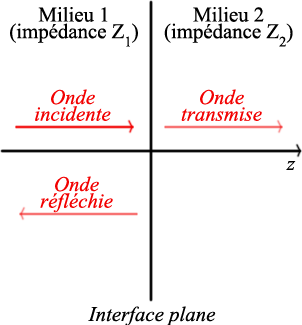
\includegraphics[scale=0.65]{ref_trans.eps}}
\end{center}

\begin{itemize}
\item Considérons une interface plane infinie entre deux fluides située en $z=0$. Une onde progressive plane émise dans la région $z < 0$ se propage dans le sens des $z$ croissants vers l'interface. Elle tombe sur l'interface sous incidence normale et elle y est en partie réfléchie et en partie transmise. L'onde réfléchie se propage dans le sens des $z < 0$, l'onde transmise dans le sens des $z > 0$.

\item On note $\overrightarrow{v}_{i}$, $p_{i}$ les champs de vitesse et de surpression associés à l'onde incidente, $\overrightarrow{v}$, $p$, ceux associés à l'onde réfléchie et enfin $\overrightarrow{v}_{t}$, $p_{t}$ ceux associés à l'onde transmise. 



\item Quand l'onde tombe sur l'interface, la composante de la vitesse normale à la surface de séparation entre les milieux est égale à gauche et à droite de celle-ci car les déplacements des fluides y sont les mêmes.

\end{itemize}

\noindent\shadowbox{\begin{minipage}[t]{1\linewidth}%
\begin{itemize}
\item Sous incidence normale, il y a continuité des champs de vitesse à l'interface:
\end{itemize}
\begin{center}
$\overrightarrow{v}_{i}(z=0,t)+\overrightarrow{v}_{r}(z=0,t)=\overrightarrow{v}_{t}(z=0,t)$
\end{center}

\end{minipage}}

\begin{itemize}
\item Dans l'approximation acoustique, l'interface peut être considérée comme fixe, ses déplacements restant faibles devant la longueur d'onde. En appliquant la relation fondamentale de la dynamique à un élément de surface dS de l'interface (de masse nulle), il vient après projection sur l'axe des $z$:
\end{itemize}

\begin{center}
$(p_{0} + p_{i} + p_{r})dS - (p_{0} + p_{t})dS = 0$
\end{center}

Ainsi, il n'existe aucune différence entre les pressions exercées par les fluides de part et d'autre de la surface.

\newpage
\noindent\shadowbox{\begin{minipage}[t]{1\linewidth}%
\begin{itemize}
\item Sous incidence normale, il y a continuité des champs de surpression à l'interface:
\end{itemize}
\begin{center}
$p_{i}(z=0,t)+p_{r}(z=0,t)=p_{t}(z=0,t)$
\end{center}
\end{minipage}}

Pour une OPPH, les différents champs considérés peuvent s'écrire en représentation complexe:
\begin{center}
$\left|\begin{array}{ccc}
\overrightarrow{\underline{v}_{i}} & = & \underline{v}_{im}e^{j(\omega t-k_{1}z)}\overrightarrow{u_{z}}\\
\underline{p}_{i} & = & \underline{p}_{im}e^{j(\omega t-k_{1}z)}
\end{array}\right.\left|\begin{array}{ccc}
\overrightarrow{\underline{v}_{r}} & = & \underline{v}_{rm}e^{j(\omega t-k_{1}z)}\overrightarrow{u_{z}}\\
\underline{p}_{r} & = & \underline{p}_{rm}e^{j(\omega t-k_{1}z)}
\end{array}\right.\left|\begin{array}{ccc}
\overrightarrow{\underline{v}_{t}} & = & \underline{v}_{tm}e^{j(\omega t-k_{2}z)}\overrightarrow{u_{z}}\\
\underline{p}_{t} & = & \underline{p}_{tm}e^{j(\omega t-k_{2}z)}
\end{array}\right.$
\end{center}

\textit{Propriété}

\noindent\shadowbox{\begin{minipage}[t]{1\linewidth}%
\begin{itemize}
\item Pour une OPPH, les \textbf{conditions aux limites à l'interface $(z=0)$} se traduisent par deux relations entre les amplitudes des champs de vitesse et de surpression:
\end{itemize}
\begin{center}
$\begin{cases}
\underline{v}_{im}+\underline{v}_{rm} & =\underline{v}_{tm}\\
\underline{p}_{im}+\underline{p}_{rm} & =\underline{p}_{tm}
\end{cases}$
\end{center}
\end{minipage}}

\subsection{Coefficients de réflexion et de transmission en amplitude}

\begin{itemize}
\item Pour une OPPH, les relations précédentes permettent de caractériser l'interface par son coefficient de réflexion $r_{v}$ et son coefficient de transmission $t_{v}$ en amplitude des vitesses définis en $z = 0$ par:
\end{itemize}
\begin{center}
\scalebox{1.2}{$r_{v}=\frac{\underline{v}_{r}}{\underline{v}_{i}}=\frac{\underline{v}_{rm}}{\underline{v}_{im}}$} et \scalebox{1.2}{$t_{v}=\frac{\underline{v}_{t}}{\underline{v}_{i}}=\frac{\underline{v}_{tm}}{\underline{v}_{im}}$}
\end{center}

En introduisant les impédances acoustiques $Z_{1}$ et $Z_{2}$ des deux fluides, les conditions aux limites s'écrivent:
\begin{center}
$\begin{cases}
\underline{v}_{im}+\underline{v}_{rm} & =\underline{v}_{tm}\\
Z_{1}\underline{v}_{im}-Z_{1}\underline{v}_{rm} & =Z_{2}\underline{v}_{tm}
\end{cases}$
\end{center}

d'où l'on déduit le système:
\begin{center}
$\begin{cases}
1+r_{v} & =t_{v}\\
Z_{1}(1-r_{v}) & =Z_{2}t_{v}
\end{cases}$
\end{center}

\textit{Propriété}

\noindent\shadowbox{\begin{minipage}[t]{1\linewidth}%
\begin{itemize}
\item Pour une OPPH, les coefficients de réflexion $r_{v}$ et de transmission $t_{v}$ \textbf{en amplitude des vitesses}, sous incidence normale, sont à l'interface:
\end{itemize}
\begin{center}
\scalebox{1.2}{$r_{v}=\frac{Z_{1}-Z_{2}}{Z_{1}+Z_{2}}$} et \scalebox{1.2}{$t_{v}=\frac{2Z_{1}}{Z_{1}+Z_{2}}$}
\end{center}
où $Z_{1}$ et $Z_{2}$ sont les impédances acoustiques des deux fluides.
\end{minipage}}

On remarque tout d'abord que ces coefficients sont réels puisque les impédances $Z_{1}$ et $Z_{2}$ le sont. Le coefficient de transmission $t_{v}$ est toujours positif: les ondes incidente et transmise vibrent toujours en phase. Le coefficient de réflexion $r_{v}$ peut être négatif: les ondes incidente et réfléchie vibrent soit en phase, soit en opposition de phase.

En outre, la réflexion est d'autant plus faible et la transmission d'autant plus grande que les impédances des milieux sont proches. Ainsi, si $Z_{1}=Z_{2}$, on a $r_{v} = 0$ et $t_{v} = 1$ : l'onde est totalement transmise, ce qui constitue une situation dite \textbf{d'adaptation d'impédances.}

\textit{A contrario}, si $Z_{2} = \infty$ (cas d'un Milieu 2 de compressibilité nulle), $r_{v} = -1$ et $t_{v} = 0$ : l'onde est totalement réfléchie. De même, si $Z_{2} = 0$ (cas d'un Milieu 2 identique au vide), il ne peut pas y avoir de propagation : l'onde est donc totalement réfléchie.

\textit{Définitions}

\noindent\shadowbox{\begin{minipage}[t]{1\linewidth}%
\begin{itemize}
\item Il est également possible de définir un coefficient de réflexion $r_{p}$ et un coefficient de transmission $t_{p}$ en amplitude des surpressions par:
\end{itemize}
\begin{center}
\scalebox{1.2}{$r_{p}=\frac{\underline{p}_{r}}{\underline{p}_{i}}$} et \scalebox{1.2}{$t_{p}=\frac{\underline{p}_{t}}{\underline{p}_{i}}$}
\end{center}

\begin{itemize}
\item Identiquement aux calculs de $r_{v}$ et $t_{v}$ (les rôles de $Z_{1}$ et $Z_{2}$ étant inversés), pour une OPPH, les coefficients de réflexion $r_{p}$ et de transmission $t_{p}$ \textbf{en amplitude des surpressions}, sous incidence normale, sont à l'interface:
\end{itemize}

\begin{center}
\scalebox{1.2}{$r_{p}=\frac{Z_{2}-Z_{1}}{Z_{1}+Z_{2}}$} et \scalebox{1.2}{$t_{p}=\frac{2Z_{2}}{Z_{1}+Z_{2}}$}
\end{center}

\end{minipage}}

\subsection{Coefficients de réflexion et de transmission en puissance}

\begin{itemize}
\item Il est également possible de caractériser l'interface par des coefficients de réflexion $R$ et de transmission $T$ des puissances sonores qui s'expriment en fonction des puissances surfaciques moyennes incidente $P_{i}$, réfléchie $P_{r}$ et transmise $P_{t}$:
\end{itemize}

\begin{center}
\scalebox{1.2}{$R=\frac{P_{r}}{P_{i}}$} et \scalebox{1.2}{$T=\frac{P_{t}}{P_{i}}$}
\end{center}

\begin{itemize}
\item La puissance surfacique moyenne échangée par l'onde est égale à la valeur moyenne temporelle $\left\langle \Pi\right\rangle$ du vecteur densité de courant d'énergie. On a:
\end{itemize}

\begin{center}
\scalebox{1.2}{$\left\langle \Pi\right\rangle =\frac{\rho_{0}c}{2}v_{m}^{2}$} avec $Z = \rho_{0}c$.
\end{center}

Pour une OPPH, il en vient:
\begin{center}
\scalebox{1.2}{$P_{i}=\frac{Z_{1}}{2}\left|\underline{v}_{im}\right|^{2}$, $P_{r}=\frac{Z_{1}}{2}\left|\underline{v}_{rm}\right|^{2}$ et $P_{t}=\frac{Z_{1}}{2}\left|\underline{v}_{tm}\right|^{2}$}
\end{center}
avec $\underline{v}_{rm}=r_{v}\underline{v}_{im}$ et $\underline{v}_{tm}=t_{v}\underline{v}_{im}$

\textit{Définition}

\noindent\shadowbox{\begin{minipage}[t]{1\linewidth}%
\begin{itemize}
\item Pour une OPPH, les coefficients de réflexion $r$ et de transmission $t$ \textbf{des puissances sonores}, sous incidence normale, s'écrivent:
\end{itemize}
\begin{center}
\scalebox{1.2}{$\begin{cases}
R=r_{v}^{2} & =\left(\frac{Z_{1}-Z_{2}}{Z_{1}+Z_{2}}\right)^{2}\\
T=t_{v}^{2}\frac{Z_{2}}{Z_{1}} & =\frac{4Z_{1}Z_{2}}{(Z_{1}+Z_{2})^{\text{2}}}
\end{cases}$}
\end{center}
Ces coefficients ne sont pas indépendants l'un de l'autre puisque $R+T=1$.
\end{minipage}}

La dernière relation ne fait que traduire la conservation de l'énergie en l'absence de phénomènes dissipatifs: l'énergie incidente est pour une part réfléchie, pour l'autre part transmise.

Comme pour les coefficients en amplitude, une onde sonore est d'autant mieux transmise d'un point de vue énergétique que les impédances des fluides sont proches. Cette propriété est exploitée, par exemple, en échographie médicale. En effet, bien que l'adaptation d'impédances ne puisse être satisfaite, un gel déposé sur le corps assure une meilleure transmission des ondes ultra-sonores.

\textit{A contrario}, il peut également être intéressant de limiter la transmission d'un son, par exemple pour mettre en place un système d'isolation phonique. On travaille alors avec des milieux d'impédances très différentes: un fluide gazeux ($Z$ de l'ordre de $10^{2}$ $kg\cdot m^{-2}\cdot s^{-1}$) et un solide ($Z$ de l'ordre de $10^{6}$ $kg\cdot m^{-2}\cdot s^{-1}$), l'onde sonore incidente prenant naissance dans le gaz. En tombant sur le solide, l'onde est presque totalement réfléchie.

\newpage
\section{Application sous forme d'un exercice}

\begin{doublespace}
Encore un autre paragraphe.
\end{doublespace}

\end{document}
